\begin{center}
  \textbf{\Huge Slutinlämning}\\[1cm]
\end{center}
\section{Implementationsbeskrivning}
\subsection{Milstolpar}
1. Förarbete\\
Fullständigt implementerad.\\
2. Kartgrafik\\
Fullständigt implementerad, främst i PlayingField.\\
3. Grafik.\\
Objekt har själva en render-funktion som ritar ut sig själva. Testfunktionerna utfasade i slutprodukten.\\
4. Fysik/spelmotor.\\
Fullständigt implementerad i physicsEngine-klassen.\\
5. Input.\\
Förflyttningsknappar, sikte, hoppa och skjut implementerat. Melee struket och sikte tillagt. Funktionalitet ligger i PlayerCommand och Player.\\
6. Winning conditions.\\
Fullständigt implementerad, bl.a. i World.\\
7. GUI\\
8. Grundläggande spel klart.\\
9. Ytterligare funktionalitet.\\
Ej implementerade.\\
\subsection{Dokumentation för programkod}
\subsubsection{KasfeqGame}
Klassen implementerar interfacet Game från Slick2D som bland annat ger oss tillgång till funktionerna init, update och render.\\
Den här klassen gör själv inget mer än att ge parametrarna till fönstret och hålla reda på den nuvarande aktiva komponenten. I detta fall är det tänkt att det ska finnas två komponenter som kan vara aktiva i KasfeqGame. Eftersom man inte både kan spela spelet och ha menyen öppen samtidigt så använder vi ett fält för att välja vilket ``tillstånd'' man är i. Den första komponenten är menyn, som ej är implementerad. Den andra komponenten är World klassen som representerar ett aktivt spel.\\
En spelkomponent implementerar minst interfacet GameComponent, men kan även implementera det utökade interfacet DrawableGameComponent som även har en funktion för utritning.\\
\subsubsection{GameComponent}
Interfacet GameComponent är grunden till alla komponenter i spelet och ger tillgång till tre funktioner: init, update och dispose.\\
\paragraph{init}
Init anropas då komponenten initieras och är vanligtvis då spelet startar.\\
\paragraph{update}
Update anropas varje frame innan något ritas ut på skärmen. Andra parametern är en integer som representerar antalet milisekunder från sista update anropet.\\
\paragraph{dispose}
Denna funktion har ingen direkt representation i Slick2D men det är tänkt att funktionen anropas innan komponenten slutar användas.\\
\subsubsection{DrawableGameComponent}
En utökning av interfacet GameComponent.
\paragraph{render}
Render anropas efter att alla update anrop är klara och skickar med ett Graphics objekt som andra parameter för utritning.\\
\subsubsection{World}
Klassen World representerar ett aktivt spel (Icke meny) och är samlingspunkten för all utritning och spellogik.\\
World håller även reda på alla aktiva (Icke döda) spelare och avslutar spelet när det finns <=1 kvar.\\
\subsubsection{GameObjectManager}
GameObjectManager klassen håller reda på alla spelobjekt. Den har även ansvaret att anropa fysikmotorn så att denna gör sitt jobb.\\
När GameObjectManager.update anropas så anropar denna GameObject.update för alla aktiva objekt. Man kan tänka sig GameObjectManager som en ``proxy'' som skickar vidare alla funktionsanrop till alla spelobjekt.\\
\subsubsection{InputManager}
InputManager klassen är ansvarig för att binda tangentbordsknappar till olika handlingar för de olika spelarna.\\
För nuvarande så är spelkontrollerna hårdkodade i koden.\\
InputManager använder sig av flera interface från Slick2D biblioteket. I grunden så binder InputManager en instans utav interfacet Control (Slick2D) till en instans av PlayerCommand klassen.\\
\subsubsection{PlayerCommand}
PlayerCommand representerar kombinationen av en spelarhandling (PlayerCommand.InputType) och ett id för den spelaren som spelarhandling är kopplad till.\\
När InputManager får ett anrop från Slick2D att en tangent blivit nertryckt så får den också PlayerCommand-objektet kopplad till den tangenten. PlayerCommand hämtar det spelobjekt som har samma ID som PlayerCommand-objektet är bundet till och anropar funktionerna som representerar handlingen som ska ske.\\
\subsubsection{PlayingField}
PlayingField klassen representerar en spelkarta och dess spelinställningar.\\
\subsubsection{Vector2d}
Vector2d klassen är en wrapper till Slick2Ds Vector2f, vi skapade den här klassen så att vi skulle slippa många casts från doubles till floats i PhysicsEngine klassen. Den här klassen är även byggd på ett sånt sätt så att den inte är in-place för att minimera mistag gjorda med referenser till vektorer.\\
\subsubsection{GameObject}
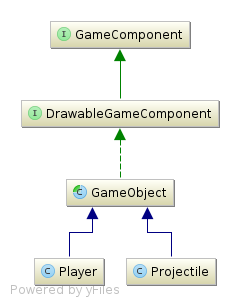
\includegraphics[scale=0.5]{gameobject}\\
GameObject klassen är en abstrakt klass som representerar alla spelobjekt och inehåller många av fälten som används av PhysicsEngine klassen för att göra beräkningar.\\
\subsubsection{Player}
Player klassen representerar en spelare.\\
\subsubsection{Projectile}
Projectile klassen representerar ett skott.\\
\subsubsection{PhysicsEngine}
PhysicsEngine klassen är fysikmotorn i spelet.\\
\subsubsection{AbstractGameLogic}
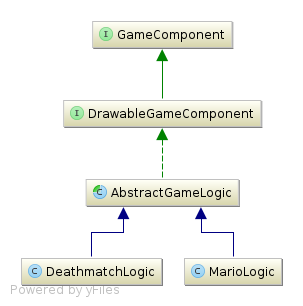
\includegraphics[scale=0.5]{gameLogics}\\
En abstrakt klass som representerar själva logiken i spelet.\\
\subsubsection{DeathmatchLogic}
En konkret implementation av en Deathmatch logik, detta är den logik som används.\\
\subsubsection{MarioLogic}
En konkret implementation av en spellogik där enda sättet att döda motståndaren är att hoppa på dem. Det går för nuvarande endast att använda den genom att ändra i källkoden.\\
\subsubsection{ResourceLoader<T>}
ResourceLoader interfacet representerar en inladdare som kan ladda in en resurs av typen <T> givet ett filnamn.\\
\pagebreak
\subsubsection{ResourceManager}
Håller reda på alla registrerade resursladdare och alla inladdade resurser.\\
loadResource funktionen laddar in en resurs av typen representerad av >Class objektet i första parametern< givet ett filnamn. Om en resurs med samma filnamn redan är inläst så kommer denna att returneras.\\
\subsubsection{TiledMapLoader}
En klass som implementerar ResourceLoader<TiledMap> interfacet och returnerar ett TiledMap objekt som sedan används för att skapa ett PlayingField objekt. <More>\\
\subsection{Användning av fritt material}
Vi har använt oss av klassbiblioteket Slick2D för utritning av spelet. Slick2D är i sin tur baserat på klassbiblioteket LWJGL som är en java wrapper för OpenGL.
\subsection{Användning av designmönster}
1. Factory Method\\
Detta mönster är uppbygt utav ett interface eller en funktion som returnerar en ny instans utav ett objekt givet ett visst antal parametrar, till skilland från att direkt skapa ett objekt så kan dessa funktioner själva lägga till information till extra information till objektet som anroparen inte skulle kunnat göra utan att bryta mot abstraktionen.\\
World.spawnNewPlayer givet en spelarfärg skapar en ny spelare, hittar en fri position på kartan och lägger till spelaren till spelet.\\
ResourceLoader klassen som givet ett filnamn laddar in en resurs av en viss typ. En ResourceLoader instans är bunden till en viss typ av resurs. En TiledMapLoader laddar in ett TiledMap objekt osv\ldots ResourceManager klassen hanterar bindningen mellan resurstypen och laddaren.\\
\vspace{11pt}
2. Builder Pattern\\
Detta mönster är uppbygt av två delar. Själva direktorn som håller reda på byggarna(``Builders'') och en eller flera byggare som själva skapar objekt. Man kan se direktorn som en proxy för byggarna.\\
ResourceManager är i detta fall klassen som är direktorn och hanterar valet av vilken ``builder'' som ska väljas för inladdning av resursen. Själva ``builder'' interfacet är i detta fall ResourceLoader som implementeras av till exempel TiledMapLoader. ResourceManager har även en objektcache så att den inte laddar om samma objekt flera gånger.\\
\subsection{Användning av objektorientering}
1. Polymorphism\\
GameObject klassen är en abstrakt klass som representerar alla objekt på spelplan. Klasserna Player och Projectile ärver och utökar GameObject.\\
GameObjectManager klassen lagrar alla aktiva instanser utav GameObject klassen.\\
\vspace{11pt}
2. Enums är Objekt (i Java)\\
Detta går även att implementera i andra språk än Java men då med statiska fält i klasser.
Vi använder oss av att enums i java är objekt genom att använda detta för att lagra egenskaper för spelet/kartan (Se PlayingField.Options).\\
En enum i Java är egentligen en klass med statiska fält med instanser utav klassen, och när man skickar enums som parametrar så skickar man dessa instanser. Jämförelse görs enkelt eftersom == operatorn jämför minnesadresser.\\
Tack vare våran implementation av Options så kan vi enkelt och snyggt beskriva egenskaper och dess standardvärden. Och även enkelt ändra värden på dessa egenskaper utan att använda en Map eller liknande för lagring.\\
Nackdelen med detta är dock att Options lagras globalt, man kan alltså inte ha flera värden på samma egenskap beroende på objekt. Detta kan lösas genom att man skapar en ny klass för att endast lagra egenskaper.\\
\vspace{11pt}
3. Interfaces\\
Vi använder interfaces i flera delar av spelet. Bland de viktigaste interfacen är GameComponent, som beskriver en del av spelet som kan initieras, updateras och tas bort. En utökning av detta interface är DrawableGameComponent som även har en funktion för utritning.\\
Dessa interface implementeras utav alla spelobjekt(GameObject) men även av andra viktiga klasser som GameObjectManager, InputManager och AbstractGameLogic.\\
\pagebreak
\subsection{Motiverade designbeslut med alternativ}
1. DrawableGameComponent\\
DrawableGameComponent som från början hade namnet GameComponent skapades tidigt för att på ett enklare sätt implementera en meny i framtiden.\\
Man kan se alla komponenterna i spelet som ett träd där roten på träden ligger i KasfeqGame klassen under fältet KasfeqGame.activeComponent.\\
Skulle vi i framtiden implementera en meny så skulle denna placeras i roten på detta träd.\\
\vspace{11pt}
2. Uppdelningen av GameComponent till GameComponent och DrawableGameComponent\\
Vi valde att ta bort funktionen för utritning ur GameComponent interfacet. Vi skapade då interfaced DrawableGameComponent to utökar GameComponent och lägger till en funktion för utritning.\\
Vi gjorde detta för att på ett mer tydligt sätt beskriva klasser som implementerar dessa interface. En klass som implementerar GameComponent har alltså ingen möjlighet att rita ut saker på skärmen.\\
\vspace{11pt}
3. TiledMap\\
Eftersom det blev lite ont om tid valde vi att använda oss av Slick2D's TiledMap klass för att hantera kartan. Denna klass har färdiga funktioner för utritning och för att enkelt hämta ut information om kartan.\\
Vi wrappar ett TiledMap objekt i våran egna klass som heter PlayingField. Denna klass läser även in kartegenskaper (eng. options) och sparar dem.
\vspace{11pt}
4. PlayingField.Options och icke konstanta enums
Eftersom enums i java är objekt (Se ``Användning av objektorientering'' för förklaring) så kan vi på ett snyggt och enkelt sätt spara kartalternativ. Nackdelen med detta är dock att dessa egenskaper är globala, alltså det går inte att ha flera PlayingField objekt för då skrivs egenskaperna över.
\pagebreak
\section{Användarmanual}
LWJGL (Lightweight java-game library) och Slick2D är dependencies.\\
\vspace{11pt}
Kontrollerna är hårdkodade i inputManager-klassen (planerade feature att lägga detta i en konfigurationsfil) och är för nuvarande\\
\vspace{11pt}
Spelare 1:\\
Sikta motsols: W\\
Sikta medsols: S\\
Vänster: A\\
Höger: D\\
Skjut: G\\
Hoppa: H\\
\vspace{11pt}
Spelare 2:\\
Sikta motsols: upp\\
Sikta medsols: ned\\
Vänster: vänster\\
Höger: höger\\
Skjut: Ins (numpad 0 med num lock avslaget)\\
Hoppa: Del (numpad , med num lock avslaget)\\
\vspace{11pt}
Men dessa går såklart att ändra i källkoden. Lista över tillgängliga knappar finns på \url{http://www.java-gaming.org/index.php?topic=27994.0}.\\
\vspace{11pt}
\vspace{11pt}
Även namnet på kartfilen är hårdkodat, i World-klassen. Detta är också planerat att läggas i en konfigurationsfil och är för nuvarande default.tmx .\\
För att ändra och skapa kartfiler används Tiled ( \url{http://www.mapeditor.org/} ) och inställningar för gravitation, friktion etc kan ställas in där.\\
\vspace{11pt}
Ovanför varje spelare finns en health bar, som krymper när man tar skada. Man tar skada genom att träffas av skott <samt bli hoppad på?>. När mätaren når botten förlorar man ett liv och spelaren återskapas på en slumpmässig plats på kartan. Siffran till vänster om mätaren är antalet liv man har kvar (alt. antalet gånger man kan återskapas). När man dör med 0 liv återskapas man inte och är ute ur matchen. När endast en spelare återstår tar spelet slut och vinnaren skrivs ut på skärmen. Sedan startar spelet om några sekunder senare.\\
\pagebreak
Röd terräng är förstörbar och går sönder om man skjuter på den.\\
\vspace{11pt}
Man kan hoppa om man står på fast mark (röd, grön eller slutet på kartan). Det går även att ``vägghoppa'' (eng. wall jump) genom att nudda en vägg åt en sida, styra i motsatt riktning samt hoppa samtidigt, detta är dock ganska svårt att få till.\\
\subsection{Instruktioner till Tiled map editor}
Dessa instruktioner är endast för att anpassa kartor till våra spel inte till hur man använder Tiled.\\
När man skapar kartor för vårat spel så finns det några viktiga regler som man måste följa.\\
Kartan måste vara skapad med följande inställningar:\\
Orientation: Orthogonal\\
Layer format: Base64 (uncompressed) eller Base64 (gzip compressed). Detta är ett krav av Slick2Ds TiledMap klass.\\
\vspace{11pt}
Lagret som används för att skapa kartan(``Tile Layer'') måste heta ``Tile Layer 1'' eller så måste en global kartparameter skapas(Map->Map Properties) men namnet ``MAPLAYER'' och namnet på lagret som värde.\\
\vspace{11pt}
När man har laddat in en tileset så och börjar skapa en karta så är det viktigt att veta att vårat spel interpreterar olika tiles som olika sorters terräng.\\
\vspace{11pt}
Följande kopplingar finns mellan id på en tile och dess funktion, där 1 är tilen mest till vänster och 3 den mest till höger i tilesettet.\\
1. Icke Förstörbar terräng\\
2. Tomhet\\
3. Förstörbar terräng\\
\vspace{11pt}
Spelet kommer endast att ladda in kartan som heter ``default.tmx'' som är placerad i mappen ``resources''. Detta betyder att man måste manuelt byta namn på kartan så att den har korrekt filnamn.\\
\subsection{Skärmdumpar}
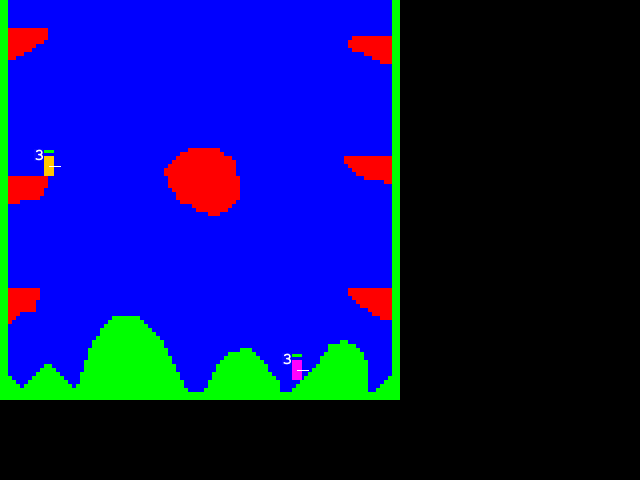
\includegraphics[scale=0.7]{game_1}\\
Nytt spel där ingen terräng är förstörd och spelarna har fullt liv och har ej tappat några liv.\\
\vspace{11pt}
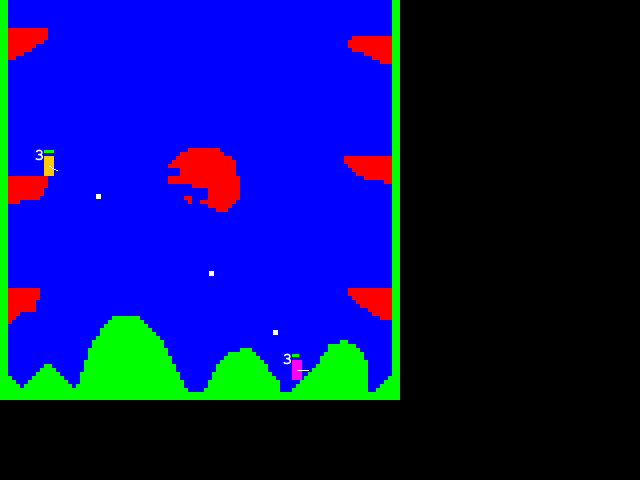
\includegraphics[scale=0.7]{game_2}\\
En bit in i spelet där spelare 2 (lila) har tappat liv, samt lite terräng är förstörd i mitten.\\
\vspace{11pt}
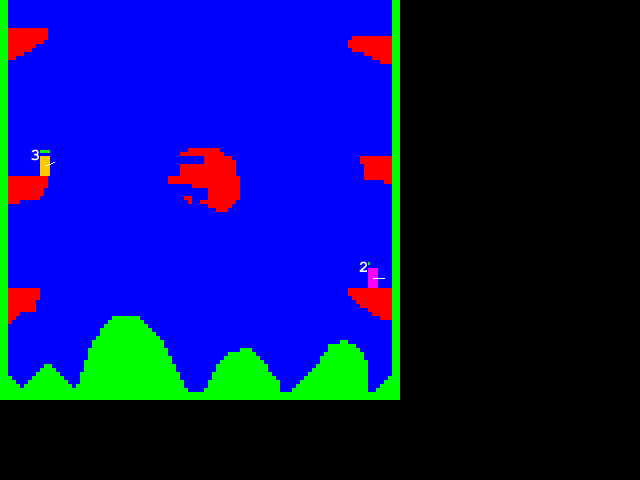
\includegraphics[scale=0.7]{game_3}\\
Ytterligare terräng är förstörd och spelare 2 (lila) är skadad samt har tappat ett liv (nere på två liv).\\
\vspace{11pt}
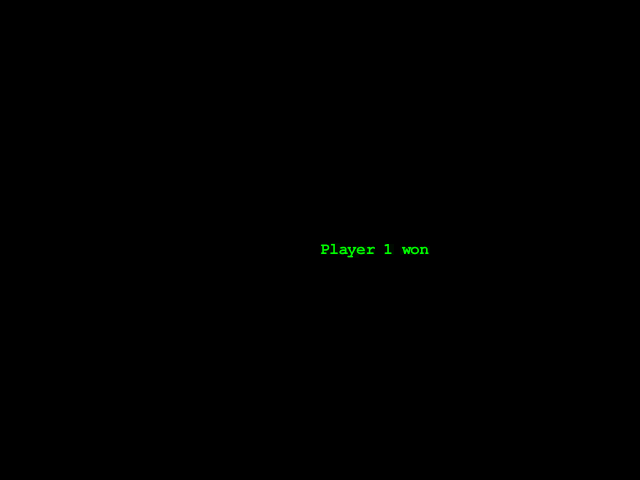
\includegraphics[scale=0.7]{game_5}\\
Spelet slut, och spelare 1 (gul) vann.\\
\section{Betygsambitioner}
Vi nöjer oss med en trea, vi har säkert en drös med objektorienterade beslut liggandes på lager men vi kommer inte på dem och uppfyller därmed inte kraven för antalet objektorienterade beslut.
\section{Utvärdering och erfarenheter}
{\color{red}
Vad gick bra? Mindre bra?\\}
I början av projektet hade vi väldigt storslagna planer på hur vi skulle göra ett helt modulärt spel där användaren lätt skulle kunna byta ut centrala delar av programmet. Detta var dock mer än vi klarade av och vi spenderade mycket tid på att planera hur abstraheringen skulle se ut, dock inte tillräckligt och när vi satte oss ned för att programmera var det fortfarande många frågetecket kvar. Det slutade med att vi två veckor innan deadline knappt hade någon kod skriven och vi kom fram till att det inte skulle gå. Vi skippade majoriteten av all modularitet vilket gjorde abstraheringen mycket enklare, och kunde således koncentrera oss på att skriva koden. Det blev stressigt mot slutet men vi lyckades hinna klart med den grundläggande delen av spelet. \\

{\color{red}Lade ni ned för mycket/lite tid?\\}
De första veckorna la vi ned alldeles för lite tid, vilket bl.a. berodde på att det var så svårt att skriva och att man inte kom någonstans när man skrev, så det var inte kul att kod. De sista veckorna la vi ned mycket mer tid och gjorde stora framsteg vilket var kul. Sett på det stora hela så hade vi nog gärna lagt ned mer tid och implementerat mer funktioner.\\

{\color{red}Var arbetsfördelningen jämn? Om inte: Vad hade ni kunnat göra för att förbättra den?\\}
Arbetsfördelningen var relativt jämn. Mikael gjorde nog lite mer då han är mer erfaren programmerare inom objektorientering och John hade assistentjobb och annat som hjälpte till att ta tid och ork ur honom.\\

{\color{red}Har ni haft någon nytta av projektbeskrivningen? Vad har varit mest användbart med den? Minst?\\}
Vi har nog nästan inte haft någon nytta av projektbeskrivningen. Vi planerade nog lite mer och specade hur spelet skulle bli, men då vi kommunicerade mycket med varandra tittade vi sällan på projektbeskrivningen. \\

{\color{red}Vad har varit mest problematiskt, om man utesluter den programmeringstekniska delen?\\}
Mest problematiskt har varit att finna motivation och tid. Då vi använt Slick2D och lwjgl har vi heller inte kunnat koda och testa på skoldatorerna, men det har inte varit något större problem annat än på redovisningspass.\\
